\documentclass{article}

\usepackage{fancyhdr}
\usepackage{extramarks}
\usepackage{amsmath}
\usepackage{amsthm}
\usepackage{amsfonts}
\usepackage{tikz}
\usepackage{algpseudocode}
\usepackage{qcircuit}
\usepackage{hyperref}
\hypersetup{
    colorlinks=true,
    linkcolor=blue,
    filecolor=magenta,
    urlcolor=purple,
}
\usepackage[ruled,vlined]{algorithm2e}

\urlstyle{same}

\usetikzlibrary{automata,positioning}

%
% Basic Document Settings
%

\topmargin=-0.45in
\evensidemargin=0in
\oddsidemargin=0in
\textwidth=6.5in
\textheight=9.0in
\headsep=0.25in

\linespread{1.1}

\pagestyle{fancy}
\lhead{\hmwkAuthorName}
\chead{}
\rhead{\hmwkClass}
\lfoot{\lastxmark}
\cfoot{\thepage}

\renewcommand\headrulewidth{0.4pt}
\renewcommand\footrulewidth{0.4pt}

\setlength\parindent{0pt}

%
% Create Problem Sections
%

\newcommand{\enterProblemHeader}[1]{
    \nobreak\extramarks{}{Problem \arabic{#1} continued on next page\ldots}\nobreak{}
    \nobreak\extramarks{Problem \arabic{#1} (continued)}{Problem \arabic{#1} continued on next page\ldots}\nobreak{}
}

\newcommand{\exitProblemHeader}[1]{
    \nobreak\extramarks{Problem \arabic{#1} (continued)}{Problem \arabic{#1} continued on next page\ldots}\nobreak{}
    \stepcounter{#1}
    \nobreak\extramarks{Problem \arabic{#1}}{}\nobreak{}
}

\setcounter{secnumdepth}{0}
\newcounter{partCounter}
\newcounter{homeworkProblemCounter}
\setcounter{homeworkProblemCounter}{1}
\nobreak\extramarks{Problem \arabic{homeworkProblemCounter}}{}\nobreak{}

%
% Homework Problem Environment
%
% This environment takes an optional argument. When given, it will adjust the
% problem counter. This is useful for when the problems given for your
% assignment aren't sequential. See the last 3 problems of this template for an
% example.
%
\newenvironment{homeworkProblem}[1][-1]{
    \ifnum#1>0
        \setcounter{homeworkProblemCounter}{#1}
    \fi
    \section{Problem \arabic{homeworkProblemCounter}}
    \setcounter{partCounter}{1}
    \enterProblemHeader{homeworkProblemCounter}
}{
    \exitProblemHeader{homeworkProblemCounter}
}

%
% Homework Details
%   - Title
%   - Due date
%   - Class
%   - Section/Time
%   - Instructor
%   - Author
%

\newcommand{\hmwkTitle}{Homework\ \#6}
\newcommand{\hmwkDueDate}{May 29th 2020}
\newcommand{\hmwkClass}{Intorduction to Quantum Computing}
\newcommand{\hmwkAuthorName}{Jakub Filipek}

%
% Title Page
%

\title{
    % \vspace{in}
    \textmd{\textbf{\hmwkClass:\ \hmwkTitle}}\\
    \normalsize\vspace{0.1in}\small{Due\ on\ \hmwkDueDate}\\
}

\author{\hmwkAuthorName}
\date{}

\renewcommand{\part}[1]{\textbf{\large Part \Alph{partCounter}}\stepcounter{partCounter}\\}

%
% Various Helper Commands
%

% Useful for algorithms
\newcommand{\alg}[1]{\textsc{\bfseries \footnotesize #1}}

% For derivatives
\newcommand{\deriv}[1]{\frac{\mathrm{d}}{\mathrm{d}x} (#1)}

% For partial derivatives
\newcommand{\pderiv}[2]{\frac{\partial}{\partial #1} (#2)}

% Integral dx
\newcommand{\dx}{\mathrm{d}x}

% Alias for the Solution section header
\newcommand{\solution}{\textbf{\large Solution}}

% Probability commands: Expectation, Variance, Covariance, Bias
\newcommand{\E}{\mathrm{E}}
\newcommand{\Var}{\mathrm{Var}}
\newcommand{\Cov}{\mathrm{Cov}}
\newcommand{\Bias}{\mathrm{Bias}}

\newcommand{\norm}[1]{\left\lVert#1\right\rVert}

\newcommand{\bra}[1]{\langle#1|}
\newcommand{\ket}[1]{|#1\rangle}
\newcommand{\qbra}{\bra{\psi}}
\newcommand{\qket}{\ket{\psi}}


\newcommand{\qwxo}[2][-1]{\ar @{-} [#1,0]|*+<2pt,4pt>[Fo]{#2}}

\begin{document}

\maketitle

% \pagebreak

\begin{homeworkProblem}
    \subsection*{Part (a)}

    Firstly, let us assume that we have 1 ancilla qubit used for the encoding of values $x_j$.
    Hence, we can encode negative values, and we can think of a first qubit as a sign qubit fo simplicity.
    Hence, whenever, a value sinks below 0, we will get $\ket{1}$ in the first register.

    \begin{algorithm}[H]
        \SetAlgoLined
        \KwResult{Index of the minimal element with probability $p = \frac{1}{2}$}
        Let $n = \log_2N$ \\
        Let $O_f\ket{\psi_{0, 1, ..., n - 1}} = \ket{\psi_0}$\\
        Let $\text{mid} = -\frac{N}{2}$\;
        \For{i = 0 to n}{
            Let success = -1\;
            \For{j = 0 to k}{
                Prepare State $\sum\limits_j \ket{j}\ket{0}$\\
                Apply $O_{mem}$. ($\sum\limits_j \ket{j}\ket{x_j}$)\\
                Add mid to the second register ($\sum\limits_j \ket{j}\ket{x_j + \text{mid}}$)\\
                Let $r$ be a result of a random Grover search using $O_f$ (i.e. either 0, or 1)\\
                \If{r == 1}{
                    success = 1\;
                    \textbf{break}\;
                }
            }
            mid = mid + success $\cdot \frac{N}{2^{i + 1}}$\;
        }
         \caption{Find Minimum Element Algorithm}
    \end{algorithm}

    From the above algorithm we can see that there are $O(k\log N\log N)$ queries to $O_{mem}$, where first $\log N$ is due to outer loop,
    and second due to the Random Grover Search which actually goes more like $\log\sqrt{N}$.
    We have to tune value of $k$ such that the overall probability of returning a correct answer is $\frac{1}{2}$. \\
    Let $x$ be a probability of success correct answer of single iteration of outer for loop. Then:
    \begin{align*}
        \frac{1}{2} &= x^{\log_2 N} \\
        \log_2{\frac{1}{2}} &= \log_2{x}\log_2 N \\
        -\frac{1}{\log_2 N} &= \log_2{x} \\
    \end{align*}
    Since, as mentioned in class random grover search has success probability of $\frac{3}{4}$. Then:
    \begin{align*}
        x &= 1 - (\frac{3}{4})^k \\
        \log_2 x &= \log_2(1 - \frac{3}{4}^k) \\
    \end{align*}

    Combining both equations we get:
    \begin{align*}
        \log_2(1 - (\frac{3}{4})^k) &= -\frac{1}{\log_2 N} \\
        1 - (\frac{3}{4})^k &= 2^{-\frac{1}{\log_2 N}} \\
        (\frac{3}{4})^k &= 1 - 2^{-\frac{1}{\log_2 N}} \\
        k\log_2(\frac{3}{4}) &= \log_2(1 - 2^{-\frac{1}{\log_2 N}}) \\
        k &= \frac{\log_2(1 - 2^{-\frac{1}{\log_2 N}})}{\log_2(\frac{3}{4})} \\
    \end{align*}

    We see that $k(N)$ is subpolynomial (as shown on Fig.~\ref{fig:p1a}).
    \begin{figure}[h]
        \centering
        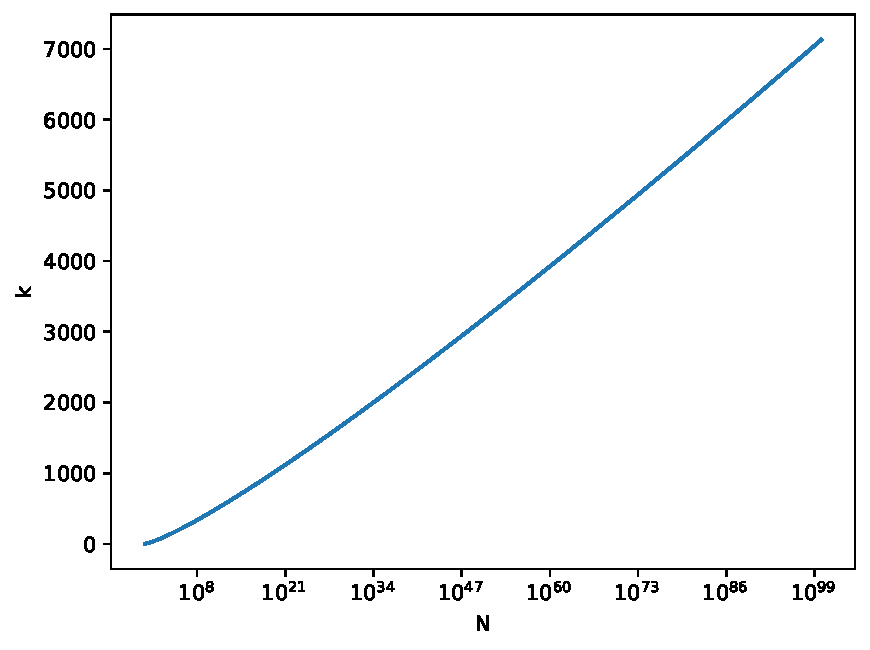
\includegraphics[scale=0.65]{p1a.pdf}
        \caption{Plot of $k$ with respect to $N$}
        \label{fig:p1a}
    \end{figure}

    Since logarithms raised to arbitrary (constant) power are faster (in asymptotic notation) than polynomials, we get:
    $\log^N k \in O(\sqrt{N})$.

    Hence overall number of queries to $O_{mem} \in O(k\log N\log N) \in O(\sqrt{N}\log N)$.

    \paragraph*{}
    \textit{Note:} The overall runtime of the algorithm is still actually worse than $O(\sqrt{N}\log{N})$,
    since Random Grover algorithm requires close to $O(\sqrt{N})$ queries to $O_f$.

    \subsection*{Part (b)}
    Let us prove that by contradiction. Assume that there exists an algorithm, which can perform a search of smallest element faster than $\Omega(\sqrt{N})$.

    Let us imagine that a specific problem is to find the smallest element of an array of all $1$'s, but a single $0$ at index $m$.
    This way the lowest value is at the index $m$.
    Then, by applying an $X$ gate to every register, we can frame it as a marked item search problem (with $1$ at index $m$).
    Thus, by finding index $m$ in the original problem, we would be able to find $m$ in the new problem.

    However, as mentioned in the class amplitude amplification is an optimal algorithm for the marked item problem and it is $\Omega(\sqrt{N})$.
    Hence existence of an algorithm that can find the smallest element faster than $\Omega(\sqrt{N})$ is contradictory.
    Thus, by contradiction, \textit{the number of queries needed to find the smallest element [...] is in $\Omega(\sqrt{N})$}.
\end{homeworkProblem}

\vspace{2cm}
\begin{homeworkProblem}
    \subsection*{Part (a)}
    \[\Qcircuit @C=1em @R=1.5em {
        \lstick{\ket{\psi_0}}     & \gate{X} & \ctrl{3} & \qw      & \ctrl{3} & \gate{X} & \gate{H} & \gate{X} & \ctrl{2} & \gate{X} & \gate{H} & \qw \\
        \lstick{\vdots}           & \gate{X} & \ctrl{2} & \qw      & \ctrl{2} & \gate{X} & \gate{H} & \gate{X} & \ctrl{1} & \gate{X} & \gate{H} & \qw \\
        \lstick{\ket{\psi_{n-1}}} & \gate{X} & \ctrl{1} & \qw      & \ctrl{1} & \gate{X} & \gate{H} & \gate{X} & \gate{Z} & \gate{X} & \gate{H} & \qw \\
        \lstick{\ket{0}}          & \qw      & \targ    & \gate{Z} & \targ    & \qw      & \qw      & \qw      & \qw      & \qw      & \qw      & \qw \\
    }\]

    Where the multi-controlled gates, can be decomposed into Toffoli/CNOT gates by stacking them into a V shape circuit, or using techinque by Craig Gidney described in question 2 of problem set 2.

    Lastly controlled-Z gate, can be decomposed into:
    \[\Qcircuit @C=1em @R=1.5em {
        & \ctrl{1} & \qw  & & = & & & \qw      & \ctrl{1} & \qw      & \qw \\
        & \gate{Z} & \qw  & &   & & & \gate{H} & \targ    & \gate{H} & \qw
    }\]

    \subsection*{Part (b)}
    I will use a method described by Figure 2 in \href{https://link.springer.com/chapter/10.1007%2F3-540-44679-6_55}{Okamoto and Watanabe}.

    In there the additional qubit is used to determine whether the Grover algorithm found the answer. Hence, the answer is deterministic.
    To make sure that the average runtime is $O(\sqrt{N})$, we do similar trick to Random Grover Search,
    where we exponentially increase the number of rotations for iteration.

    \subsection*{Part (c)}
    First let us introduce a classical operation $E$, which will end the whole algorithm if the input is 1, and continue otherwise.

    Let us also use W defined in part a.
    Let us also have the oracle $O_f\ket{x}\ket{c} = \ket{x}\ket{c \oplus f(x)}$, according to the one defined in the problem
    (i.e. only for $\ket{0}^{\otimes n}$ $f$ returns $1$).

    Then for iteration $i$ we have circuit:

    \[\Qcircuit @C=1em @R=1.5em {
        & \lstick{\ket{0}} & \gate{H} & \multigate{2}{W^{2^i}} & \multigate{3}{O_f} & \qw    & \qw      & \qw \\
        & \lstick{\vdots}  & \gate{H} & \ghost{W^{2^i}}        & \ghost{O_f}        & \qw    & \qw      & \qw \\
        & \lstick{\ket{0}} & \gate{H} & \ghost{W^{2^i}}        & \ghost{O_f}        & \qw    & \qw      & \qw \\
        & \lstick{\ket{0}} & \qw      & \qw                    & \ghost{O_f}        & \meter & \gate{E} & \cw \\
    }\]

    And such circuit is repeated for $i = 0, 1, 2, 3, ...$ until $E$ terminates it.

    \subsection*{Part (d)}
    I will refer to the equations 1 and 4 in \href{https://link.springer.com/chapter/10.1007%2F3-540-44679-6_55}{Okamoto and Watanabe},
    since they provide a proof for average runtime of the above algorithm to have $\frac{8\pi}{3}\sqrt{\frac{N}{t}}$.

    In case of this problem the number of solutions ($t$) is 1, since only all-zero string returns a correct answer.
    Hence the problem we have to solve is:
    \begin{align*}
        \frac{8\pi}{3}\sqrt{2^n} &= 2^n - 1 \\
        n = \lceil 6.17 \rceil &= 7
    \end{align*}

    Hence if we are supposed to use 7 or more qubits the quantum algorithm outperforms the classical (assuming similarities in all other aspects).
\end{homeworkProblem}
\end{document}